\documentclass{standalone}
\usepackage{tikz}
\usetikzlibrary{patterns, angles}

\begin{document}
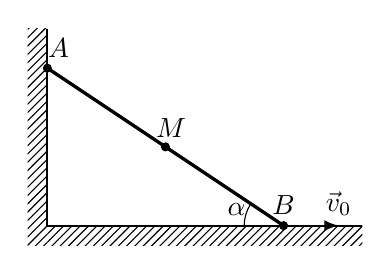
\begin{tikzpicture}
	\coordinate (A) at (0, 2);
    \coordinate (C) at (0, 2.5);
    \coordinate (O) at (0, 0);
    \coordinate (D) at (4, 0);
    \coordinate (B) at (3, 0);
    \coordinate (M) at (1.5, 1);
       
	\draw [draw=none, pattern=north east lines] (C) rectangle (-0.25,-0.25);
	\draw [draw=none, pattern=north east lines] (0,-0.25) rectangle (D);	
	\draw [thick] (C) -- (O) -- (D);
	\draw [very thick] (A) node [right=4pt, above] {$A$} -- (B) node [above] {$B$};
	\draw [fill] (A) circle (0.05);	
	\draw [fill] (B) circle (0.05);
	\draw [fill] (M) circle (0.05) node [right=2pt, above] {$M$};
	\pic [draw, -, angle eccentricity=1.5] {angle = A--B--O};
	\node [left=17pt, above] at (B) {$\alpha$};
	\draw [arrows={-latex}, thick] (B) -- (3.7, 0) node [above]  {$\vec{v}_0$};
\end{tikzpicture}
\end{document}